\subsection{Validazione} \label{validazione}

	\subsubsection{Scopo del processo}
		Il seguente processo ha lo scopo di determinare in maniera oggettiva la conformità dei requisiti e
		del prodotto software realizzato, rispetto all'uso prestabilito all'assegnazione dell'appalto come
		dimostrazione di adempimento contrattuale alla Committente.

	\subsubsection{Attività di validazione}
		La validazione può effettuarsi solo sul prodotto software ultimato; precondizione è, quindi, il
		superamento di tutti i test di unità e di integrazione, indicativi della corretta implementazione
		dell'architettura progettata.

		Sul software vengono, dunque, effettuati in maniera interna al Fornitore e da parte di Verificatori
		estranei alla loro specifica a garanzia di imparzialità, i test di sistema definiti in \vPianoDiQualifica{} §2.
		L'esito positivo coincide, come mostrato dal \glossaryItem{modello a V}, con il soddisfacimento dei
		requisiti individuati dall'attività di analisi e permette di affrontare il collaudo.

		Il collaudo è un'attività formale supervisionata dalla Committente che consiste nella dimostrazione
		pratica del software prodotto di poter superare tutti i test di accettazione concordati contrattualmente.

		Il superamento del collaudo coincide con il superamento della procedura di validazione, poiché conferma
		che i requisiti analizzati e realizzati nel software adempiono alle richieste espresse nel capitolato, e con il
		rilascio del prodotto secondo le modalità di fornitura stabilite.

		È compito del \Responsabile{} istanziare e pianificare la validazione affinché la si superi nei tempi dettati
		dal \vPianoDiProgetto{} §5.6.

		\begin{figure}[htbp]
			\centering
			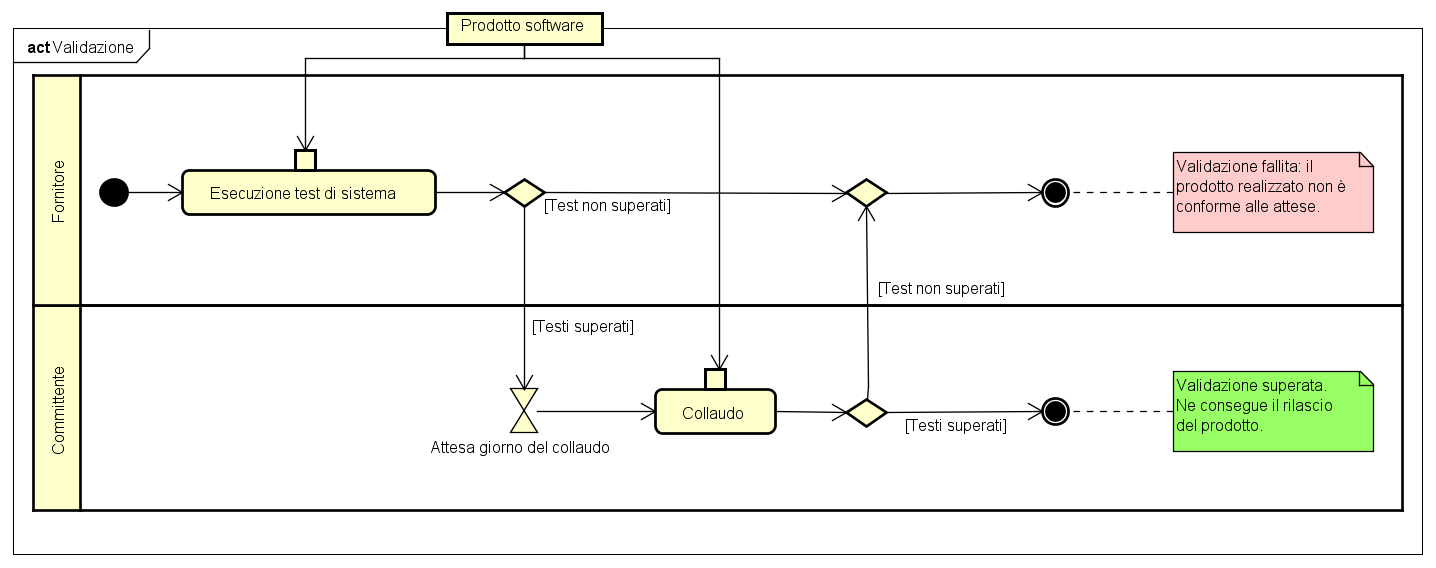
\includegraphics[scale=0.35]{./img/validazione.png}
			\caption[Procedura di validazione]{Procedura di validazione}
		\end{figure}\\